\documentclass[twocolumn,fontsize=11pt]{scrartcl}

% Basic packages
\usepackage[utf8]{inputenc}
\usepackage[T1]{fontenc}
\usepackage{lmodern}
\usepackage[a4paper,margin=1.5cm]{geometry}
\usepackage{multicol}
\usepackage{graphicx}
\usepackage{caption}
\usepackage{subcaption}
\usepackage{amsmath,amssymb}
\usepackage{siunitx}
\usepackage{booktabs}
\usepackage{physics}
\usepackage{float}
\usepackage{hyperref}
\usepackage{physics_macros} % Your custom macros
\usepackage{biblatex} % For bibliography
\addbibresource{bibliography.bib}

% Header and footer
\usepackage{fancyhdr}
\pagestyle{fancy}
\fancyhf{}
\lhead{Star and Stellar Evolution}
\rhead{\thepage}

%Folder
\graphicspath{{plots/}}

% Title
\title{\vspace{-1cm}Stellar Structure Evolution with MESA}
\author{Bruno da Rocha Schultz}
\date{\today}

\begin{document}
\maketitle

\section*{Exercise 1}

\paragraph{Q.1.1:} Why is there only one history file but multiple profile files?

\paragraph{A:} The history file contains the global properties of the star at each time step, while the profile files contain the detailed structure of the star at specific points in time. The history file is updated at each time step, but the profile files are only written at certain intervals. So there is one history file for the entire simulation, but multiple profile files corresponding to different time steps.

\paragraph{Q.1.2:} Show with a plot whether or not the size of the time steps in the history file changes
during the simulation, and discuss why.

\paragraph{A:} The time steps in the history file do change during the simulation. This is because MESA uses an adaptive time-stepping algorithm to ensure that the simulation progresses at a rate that captures the important changes in the star's structure and evolution. The time steps are smaller during rapid changes (like during a shell flash) and larger during more stable phases. Cf. Figure \ref{fig:time_steps} for a plot of the time steps recorded in the history file.

\begin{figure}[htbp]
    \centering
    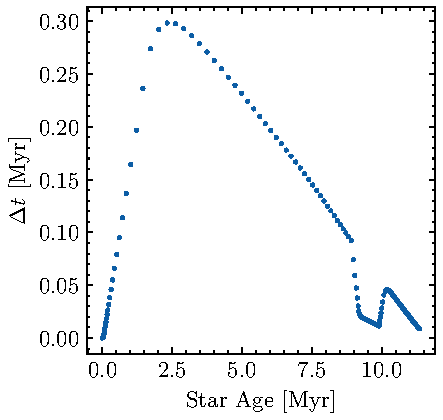
\includegraphics{dt_vs_age.pdf}
    \caption{Time steps recorded in the history file. The x-axis represents the stellar age, and the y-axis indicates the time step size. For visualization purposes, the logarithmic time step values from the history file have been converted to linear scale in this plot.}
    \label{fig:time_steps}
\end{figure}

\paragraph{Q.1.3:} Similarly, show with a plot whether or not the grid spacing in a profile file of your
choice is constant, and discuss why. From this plot, also infer which zone is the most
central zone (zone number 1 or the zone with the highest number).

\paragraph{Q.1.4:} Similarly, show with a plot whether or not the grid spacing in a profile file of your
choice is constant, and discuss why. From this plot, also infer which zone is the most
central zone (zone number 1 or the zone with the highest number).

\printbibliography

\end{document}
